\section{Time-dependent discontinuity model}
\label{section:time_problem}
For the time-dependent discontinuity problem, we change the value of the parameter $\beta$ from 0.9 to 0.005 at t=27. This introduces a discontinuity into the problem. We will show that this discontinuity leads to inaccuracies in the solutions computed by some of the solvers, particularly the fixed-step solvers. We then introduce a form of discontinuity handling, using what are known as cold starts, to show how to obtain an efficient and accurate approach for solving time-dependent discontinuity problems.

\subsection{Naive solution of the time-dependent discontinuity model}
\label{subsection:naive_time_problem}
A naive implementation of the model involves using an `if' statement inside the right-hand side function, $f(t, y)$, to implement the change in $\beta$ as measures are implemented. 

In pseudo code, this looks like:

\begin{minipage}{\linewidth}
\begin{lstlisting}[language=Python]
function model_with_if(t, y)
    // ...
    beta = 0.005
    if t < 27:
        beta = 0.9
    // ...
    // return (dSdt, dEdt, dIdt, dRdt)
\end{lstlisting}
\end{minipage}

Also, to stay true to a naive treatment, we will use the default tolerances in this section. Discrepancies across the programming environments that are due to tolerance issues are investigated in Section $\ref{subsection:time_tolerance_study}$. We also note than for the fixed step-size methods in the R environment, the step-size is 1 as the solvers will default to the distance between two consecutive output points, and we choose as our standard output point sequence $t=1, 2, \dots, 95$.

\subsubsection{Naive solution to the time-dependent discontinuity model in R}

\begin{figure}[H]
\centering
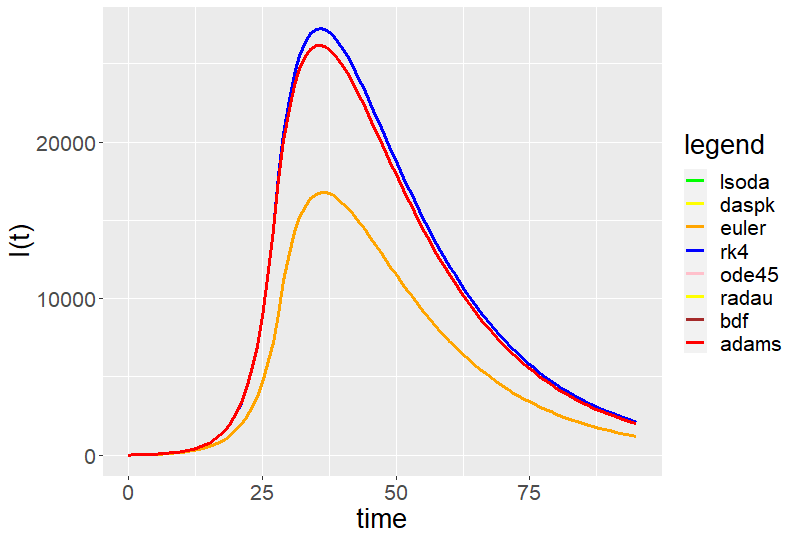
\includegraphics[width=0.7\linewidth]{./figures/time_discontinuity_R}
\caption{Solutions to the time-dependent discontinuity model using solvers from R.}
\label{fig:time_discontinuity_R}
\end{figure}

From Figure $\ref{fig:time_discontinuity_R}$, we can see that all the methods except `euler' and `rk4' compute solutions that agree to ``eyeball" accuracy, which typically means that they agree to about two significant digits. The `rk4' method gives a solution that is somewhat close to the solutions obtained by the other solvers but the solution computed by the `euler' method is noticibly inaccurate. We note that all the other methods have error control while the `rk4' and `euler' methods are fixed step-size solvers.

We also note that the `rk4' method does better than the `euler' method for this specific problem as it has a higher order. But, since `rk4' is using a fixed step-size with no error control, its performance is still better than expected. We show that this is entirely because of the issue associated with how output points are handled, as discussed in Section $\ref{subsection:solution_output_points_impl}$. If we use an output point sequence with a larger spacing between the output points, the `rk4' methods gives results that are of similar accuracy to the results yielded by the  `euler' method. Figure $\ref{fig:rk4_messing_up_no_event_R}$ shows an experiment with `rk4' used with different spacings between output points plotted together with an accurate solution (in red). We can see that as we increase the output point spacing, the solver does not give accurate results. Analyzing the source for `rk4' and `euler' shows that these methods select the step size based on the requested output points. Spacing out the output points affects the step-size which affects the accuracy of the fixed step-size solvers.

\begin{figure}[H]
\centering
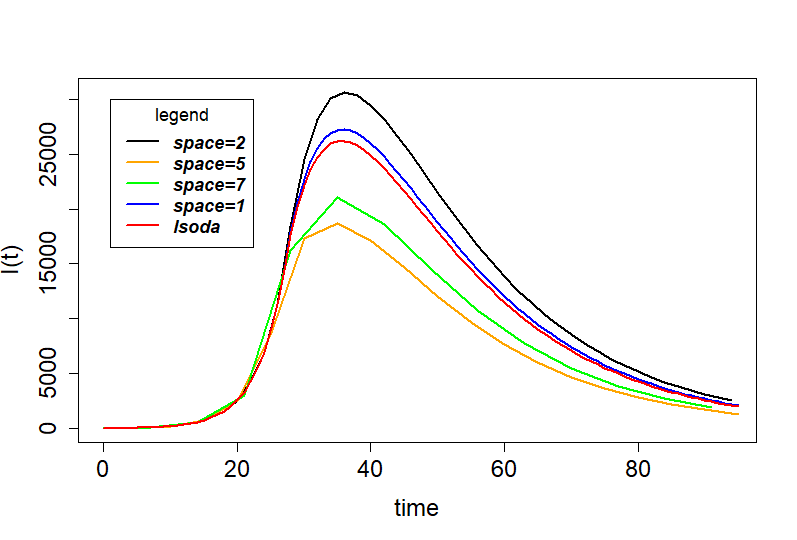
\includegraphics[width=0.7\linewidth]{./figures/rk4_messing_up_no_event_R}
\caption{Solutions computed by `rk4' in R with output point spacings compared with an accurate solution computed by LSODA.}
\label{fig:rk4_messing_up_no_event_R}
\end{figure}

If a user wants to use `rk4' or `euler', to get an accurate solution, the user would have to choose a small step-size. However, the user cannot know beforehand how small a step-size is small enough to deliver a desired accuracy. Furthermore, there is the issue that a sufficiently small step-size can vary from one part of the domain to another as the problem difficulty changes. A fixed step-size solver will have to choose the smallest step required anywhere in the domain and this can lead to substantial inefficiency. A better approach is to not use fixed step-size solvers. Reliable methods with error control should be preferred since these solvers can adaptively choose a stepsize sequence that will deliver the desired accuracy.

\subsubsection{Naive solution to the time-dependent discontinuity model in Python}
\begin{figure}[H]
\centering
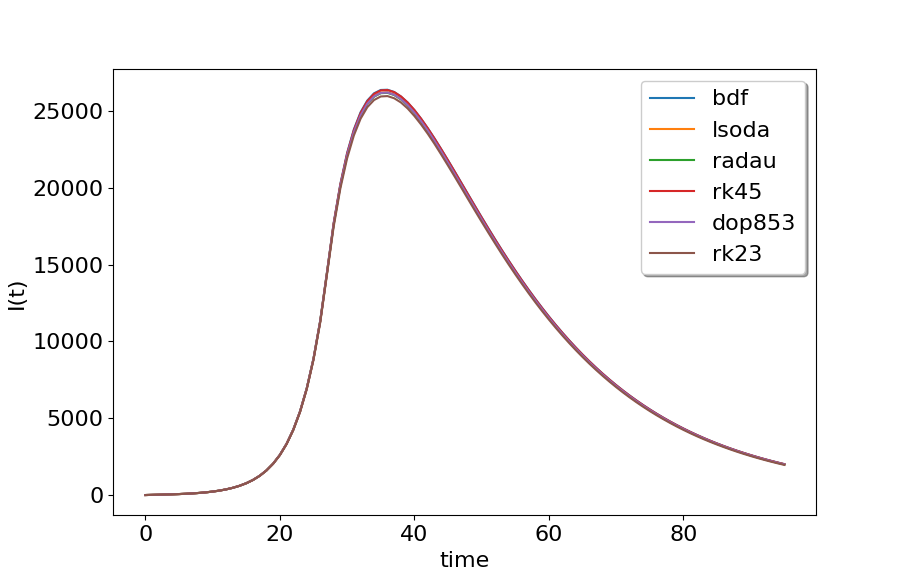
\includegraphics[width=0.7\linewidth]{./figures/time_discontinuity_py}
\caption{Solutions to the time-dependent discontinuity model using solvers from Python.}
\label{fig:time_discontinuity_py}
\end{figure}
From Figure $\ref{fig:time_discontinuity_py}$, we can see that all the methods in the Python's $solve\_ivp()$ function work reasonably well. There is some blurring at the peak, indicating some disagreement among the methods, but all the methods provide reasonably accurate results. Python only provides error-controlled solvers and thus we can see that a reasonably sharp tolerance with an error-control method is what is required to step over this type of discontinuity. (Recall that all Python methods use a default absolute tolerance of $10^{-6}$ and a relative tolerance of $10^{-3}$.)

\subsubsection{Naive solution to the time-dependent discontinuity model in Scilab}
\begin{figure}[H]
\centering
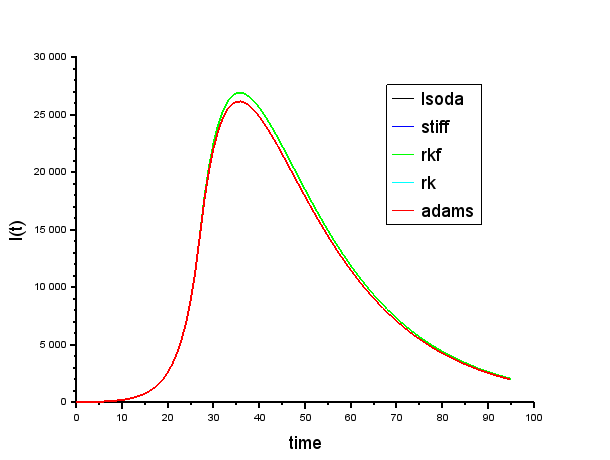
\includegraphics[width=0.7\linewidth]{./figures/time_discontinuity_scilab}
\caption{Solutions to the time-dependent discontinuity model using solvers from Scilab.}
\label{fig:time_discontinuity_scilab}
\end{figure}
From Figure $\ref{fig:time_discontinuity_scilab}$, we can see that in Scilab, all the methods give similar solutions except for `rkf'. This is interesting as we know that `rkf' uses error control. This is explained by noting that `rkf' uses coarser default absolute and relative tolerances. We will show, through a tolerance analysis in Section $\ref{subsection:time_tolerance_study}$, that with a sharp enough tolerance, `rkf' also provides a reasonably accurate solution.

The other methods are all error-controlled and give similar results as expected. We note that all of the other methods have a higher default tolerance than `rkf' and thus this result is not surprising.

These results also confirm that an error control solver with a sharp tolerance can step over this type of discontinuity.

\subsubsection{Naive solution to the time-dependent discontinuity model in Matlab}
\begin{figure}[H]
\centering
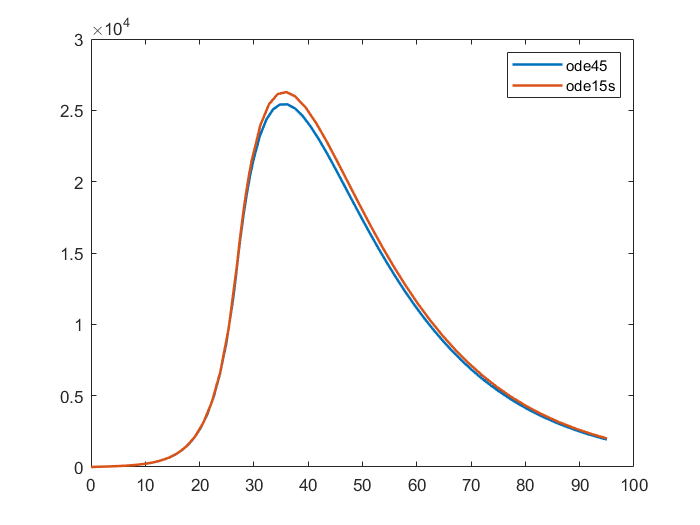
\includegraphics[width=0.7\linewidth]{./figures/time_discontinuity_matlab}
\caption{Solutions to the time-dependent discontinuity model using solvers from Matlab.}
\label{fig:time_discontinuity_matlab}
\end{figure}
Figure $\ref{fig:time_discontinuity_matlab}$ shows that Matlab's $ode45$ and $ode15s$ are not in complete agreement. This is unexpected because both are error controlled. We note that the behaviour of $ode45$ is similar to what we have seen for `rkf' in Scilab but the methods are based on different algorithms. In Matlab, both $ode45$ and $ode15s$ have the same default tolerances so we can rule out that a tolerance difference is the reason for this behavior. We will see, in Section $\ref{subsection:time_tolerance_study}$, that $ode45$ can give a similar result to $ode15s$  when the tolerance is sharp enough. From this we can suggest that the issue may be associated with differences in the way that the two solvers apply the absolute and relative tolerances.

\subsubsection{Summary of naive approach of 
solving time-dependent discontinuity problems}
Generally, the time-dependent discontinuity problem can be solved accurately by solvers that employ error control with a sufficiently sharp tolerance. However as we will see in the next section, the computations are quite inefficient. (See Section $\ref{subsection:effect_of_discontinuity}$ for an explanation of why this inefficiency arises.)

\subsection{An improved approach for the solution 
of the time-dependent discontinuity model}
\label{subsection:time_disc_handling}
A better way to solve the time-dependent discontinuity problem is to make use of cold starts. This means that we integrate up to the time at which the discontinuity arises and then after the discontinuity we continue the integration with a \emph{separate} call to the solver. Restarting a solver with a cold start at the time of the discontinuity improves the accuracy as we will see in this and the next section. It also improves the efficiency as fewer function calls are required since we do not have the spike in function calls due to the repeated step-size resizing described in Section $\ref{subsection:effect_of_discontinuity}$.

A cold start means that we restart the solver with method parameters set so that the solver starts the computation with no values from the previous computation. It will also involve using a small initial step size and for methods of varying order like the `BDF' and `Adams' methods, they will restart with the default order which is order 1.

To solve the time dependent discontinuity problem, we will integrate from time 0 to the time that measures are implemented, t=27, with one call to the solver and then use the solution values at t=27 as the initial values to make another call that will integrate (restarting with a cold start) from t=27 to $t_f$. The pseudo-code is as follows:

\begin{minipage}{\linewidth}
\begin{lstlisting}[language=Python]
initial_values = (S0, E0, I0, R0)
tspan_before = [0, 27]
solution_before = ode(intial_values, model_before_measures,
tspan_before)

initial_values_after = extract_last_row(solution_before)
tspan_after = [27, 95]
solution_after = ode(intial_values_after, 
model_after_measures, tspan_after)

solution = concatenate(solution_before, solution_after)
\end{lstlisting}
\end{minipage}

This technique can be applied to any problem where it is known when the discontinuity is introduced. {\bfseries This is a much better approach than introducing a time-dependent `if' statement into the model.}

\subsection{Solving the time-dependent discontinuity model using a cold start} 
\subsubsection{Solving the time-dependent discontinuity model in R using a cold start} 
\begin{figure}[H]
\centering
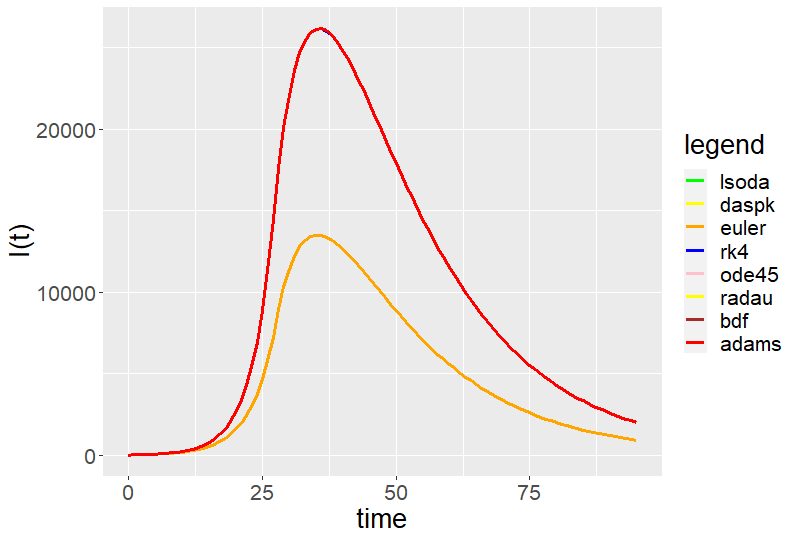
\includegraphics[width=0.7\linewidth]{./figures/solve_time_discontinuity_R}
\caption{Solutions to the time-dependent discontinuity model using solvers from R and a cold start at t=27.}
\label{fig:solve_time_discontinuity_R}
\end{figure}
From Figure $\ref{fig:solve_time_discontinuity_R}$, we see that the `euler' method still fails even when the cold start form of discontinuity handling is introduced. This is as expected as this method has no error control and thus it still suffers from accuracy issues and will require smaller steps to achieve even ``eyeball" accuracy.

We see that breaking the integration into two parts allows `rk4' perform better. The method has higher order but this exceptionally good performance is still unexpected. We will show in Figure $\ref{fig:rk4_messing_up_with_event_R}$ that the performance of `rk4' is associated with the method of handling output points as described in Section $\ref{subsection:solution_output_points_impl}$.

\begin{figure}[H]
\centering
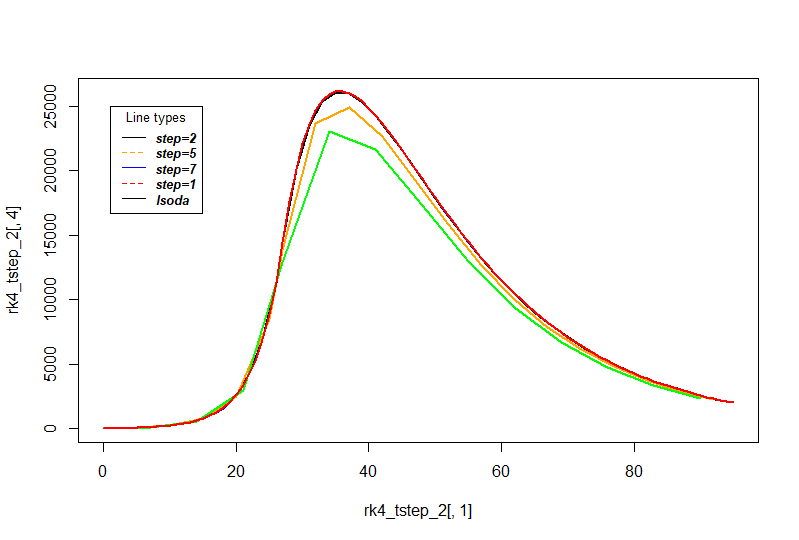
\includegraphics[width=0.7\linewidth]{./figures/rk4_messing_up_with_event_R}
\caption{The R version of `rk4' with larger spacings between the output points and with discontinuity handling.}
\label{fig:rk4_messing_up_with_event_R}
\end{figure}

Thus our recommendation to avoid fixed step size solvers still holds since users will not typically know how small the step size needs to be to obtain sufficient accuracy.

We also note again, that all the error-controlled solvers perform well. We will see, from the efficiency data, that using cold starts results in a more efficient computation. Using cold starts, the error control solvers do not have to step over the discontinuity and we will not have the spike in the number of function evaluations as we discussed in $\ref{subsection:effect_of_discontinuity}$. Table $\ref{tab:time_discontinuity_R}$ shows that discontinuity handling gnerally reduces the number of function evaluations. 

\begin{table}[H]
\caption {R efficiency data for the time-dependent discontinuity problem - number of function evaluations} 
\label{tab:time_discontinuity_R}
\begin{center}
\begin{tabular}{ c c c } 
method & no discontinuity handling & with discontinuity handling \\ 
euler & 96 & 97 \\
rk4 & 381 & 382 \\ 
lsoda & 332 & 272 \\
ode45 & 735 & 599 \\
radau & 679 & 585 \\
bdf & 423 & 263 \\
adams & 210 & 176 \\
daspk & 517 & 521
\end{tabular}
\end{center}
\end{table}

Our analysis of the efficiency data in Table $\ref{tab:time_discontinuity_R}$ starts by noting that the non-error controlled solvers in the `euler' and rk4' methods have essentially the same number of function evaluations in both cases, the additional evaluation being due to evaluating the function twice at time 27. This indicates that they are just stepping from output point to output point using the same fixed step-size both with and without the discontinuity handling.

Next, we note significant decreases in the number of function evaluations for all the remaining solvers except `daspk'. These reductions in the number of function evaluations will have a significant impact on the CPU time for the difficult problem. This is entirely explained in Section $\ref{subsection:effect_of_discontinuity}$ where the error-controlled solvers have to repeatedly resize the step-size as they encounter the discontinuity.

Finally, we explain the almost constant value of the number of function evaluations for the `daspk' method through the fact that, in the R implementation, it is not using an appropriate interpolation scheme to obtain solution approximations at the output points. Instead it is using the approach described in Section $\ref{subsection:solution_output_points_impl}$. In another experiment with a larger spacing between output points, we found that `daspk' uses 627 function evaluations without discontinuity handling and 522 function evaluations with discontinuity handling; a result that is more consistent with the results from Table $\ref{tab:time_discontinuity_R}$ for the other error control solvers.

In Section $\ref{subsection:time_tolerance_study}$, we will see that this type of discontinuity handling also allows us to use coarser tolerances, which improves the efficiency of the computation.

\subsubsection{Solving the time-dependent discontinuity model in Python using a cold start} 
\begin{figure}[H]
\centering
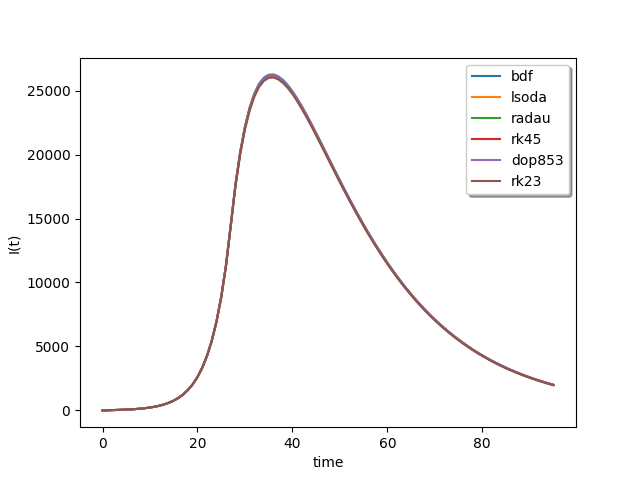
\includegraphics[width=0.7\linewidth]{./figures/solve_time_discontinuity_py}
\caption{Solutions to the time-dependent discontinuity model using solvers from Python and a cold start at t=27.}
\label{fig:solve_time_discontinuity_py}
\end{figure}
The Python solvers did not have significant accuracy issues even without discontinuity handling. This is because all the available methods use error control and the default tolerances are sharp enough. From Figure $\ref{fig:solve_time_discontinuity_py}$, we can see that the Python solvers again give sufficiently accurate results. Furthermore, the slight blurring at the peak has disappeared indicating that there is an even better agreement among the solvers. The addition of discontinuity handling also significantly reduces the number of function evaluations. This can be seen in Table $\ref{tab:time_discontinuity_Py}$.

\begin{table}[H]
\caption {Python efficiency data for the time-dependent discontinuity problem - number of function evaluations} 
\label{tab:time_discontinuity_Py} 
\begin{center}
\begin{tabular}{ c c c }
method & no discontinuity handling & with discontinuity handling \\ 
lsoda & 162 & 124 \\
rk45 & 134 & 130 \\
bdf & 202 & 146 \\
radau & 336 & 220 \\
dop853 & 329 & 181 \\
rk23 & 152 & 127 \\
\end{tabular}
\end{center}
\end{table}

The Python solvers do not allow the space between the output points to affect the accuracy. They use some form of local interpolation within each step where there are output points.

From Table $\ref{tab:time_discontinuity_Py}$, we see that when discontinuity handling is introduced, the methods use fewer function evaluations. There are some significant improvements for `BDF', `DOP853' and `Radau'. There are slight decreases for `LSODA' and `RK23' and only a very small decrease for `RK45'. 

\subsubsection{Solving the time-dependent discontinuity model in Scilab using a cold start} 
\begin{figure}[H]
\centering
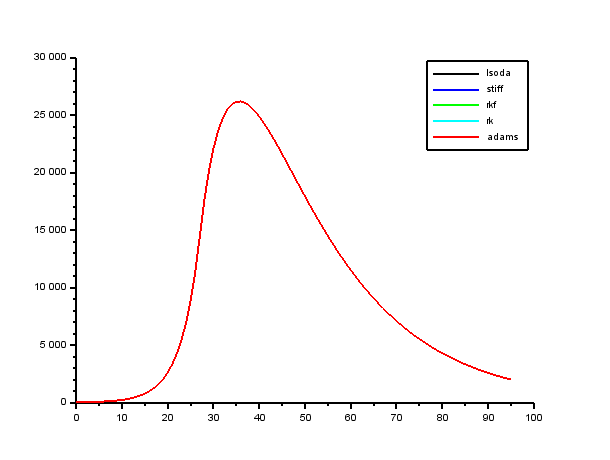
\includegraphics[width=0.7\linewidth]{./figures/solve_time_discontinuity_scilab}
\caption{Solutions to the time-dependent discontinuity model using solvers from Scilab and a cold start at t=27.}
\label{fig:solve_time_discontinuity_scilab}
\end{figure}
We can see from Figure $\ref{fig:solve_time_discontinuity_scilab}$ that all the methods show good agreement and thus the time-dependent discontinuity model is being solved to a reasonable accuracy. The `rkf' method is also giving reasonable results. This is despite `rkf' having a coarser default tolerance.

The addition of discontinuity handling also significantly reduces the number of function evaluations as seen in Table $\ref{tab:time_discontinuity_scilab}$.

\begin{table}[H]
\caption {Scilab efficiency data for the time-dependent discontinuity problem - number of function evaluations.} 
\label{tab:time_discontinuity_scilab} 
\begin{center}
\begin{tabular}{ c c c }
method & no discontinuity handling & with discontinuity handling \\ 
lsoda & 346 & 292 \\
stiff & 531 & 362 \\
rkf & 589 & 590 \\
rk & 1649 & 1473 \\
adams & 304 & 221 \\
\end{tabular}
\end{center}
\end{table}

From Table $\ref{tab:time_discontinuity_scilab}$, we see that all the methods use fewer function evaluations except for `rkf'. We see substantial decreases in the number of function evaluations for `lsoda', `stiff', `rk' and `adams'.`

The unusual result for `rkf' occurs because `rkf' is using the method for handling output points as outlined in Section $\ref{subsection:solution_output_points_impl}$. The results, when we space out the output points more, are 335 function evaluations without discontinuity handling and 292 function evaluations with discontinuity handling.

We note that the high number of function evaluations in `rk' with and without discontinuity handling is because it is using Richardson extrapolation to get an error estimate. Richardson involves using the Runge-Kutta method twice, once to get the solution approximation at the end of the step and once again with half the step-size to do two steps in the same interval to get a more accurate solution to use to obtain an error estimate. Thus in one actual step, there are three `steps' and this leads to a large number of function evaluations.

\subsubsection{Solving the time-dependent discontinuity model in Matlab using a cold start}
\begin{figure}[H]
\centering
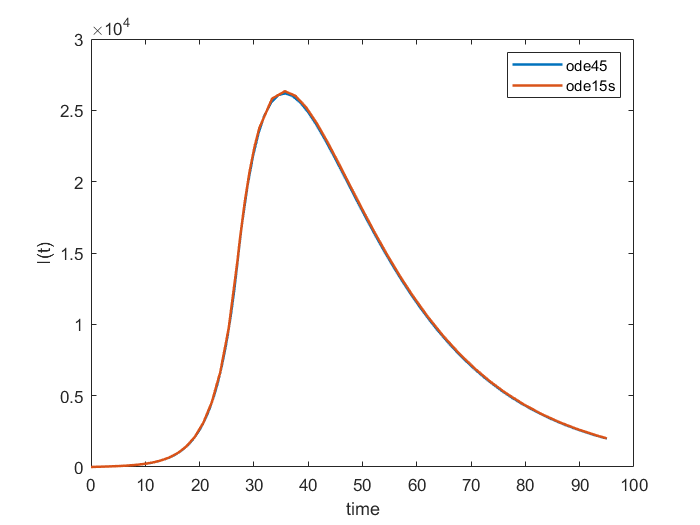
\includegraphics[width=0.7\linewidth]{./figures/solve_time_discontinuity_matlab}
\caption{Solutions to the time-dependent discontinuity model using solvers from Matlab and a cold start at t=27.}
\label{fig:solve_time_discontinuity_matlab}
\end{figure}

From Figure $\ref{fig:solve_time_discontinuity_matlab}$ we can see that both solvers give similar solutions. We remember that with an `if' statement inside the function $f(t, y(t))$, the two solvers gave somewhat different solutions. As we will show in Section $\ref{subsection:time_tolerance_study}$, the discontinuity handling allows us to use a coarser tolerance and thus allows $ode45$ to give a reasonably accurate result.

We also show in Table $\ref{tab:time_discontinuity_matlab}$ that discontinuity handling allows the solvers to use fewer function evaluations.

\begin{table}[H]
\caption {Matlab efficiency data for the time-dependent discontinuity problem - number of function evaluations} 
\label{tab:time_discontinuity_matlab} 
\begin{center}
\begin{tabular}{ c c c }
method & no discontinuity handling & with discontinuity handling \\ 
ode45 & 175 & 164 \\
ode15s & 144 & 113 \\
\end{tabular}
\end{center}
\end{table}

From Table $\ref{tab:time_discontinuity_matlab}$, we see that $ode45$ uses 11 fewer function evaluations while $ode15s$ uses 31 fewer function evaluations.

\subsection{Efficiency data and tolerance study 
for the time-dependent discontinuity model}
\label{subsection:time_tolerance_study}
It is not uncommon for researchers to use an ODE solver in a loop or within an optimization algorithm so that they can study models with different problem-dependent parameter values. In such contexts, it may be reasonable to coarsen the tolerances when the computation is taking too long. In this section, we investigate how coarse we can set the tolerance while still obtaining reasonably accurate results for the time-dependent discontinuity model. 

We investigate `lsoda' across R, Python, and Scilab as they all appear to use the same source code. We use this experiment to show that discontinuity handling allows us to use coarser tolerances.

We will also investigate `rkf' in Scilab as it has a smaller default tolerance than the other Scilab solvers, and $ode45$ in Matlab, both of which failed to solve the time-dependent discontinuity model with an accuracy that was comparable to that of the other solvers. We will show that they can solve the problem with reasonable accuracy without discontinuity handling only at sharper tolerances than the default tolerances. We also investigate solvers based on Runge-Kutta pairs of the same order as the pair used in `rkf' and $ode45$ in the other programming environments; R and Python each have a version of DOPRI5 but do not share the same source code. The DOPRI5 in Python is a Python implementation and the one in R is an interface to a C implementation. The Matlab solver, $ode45$, uses DOPRI5 but it is implemented in the Matlab programming language.

\subsubsection{Comparing LSODA across platforms for the time-dependent discontinuity model}
\subparagraph{Time-dependent discontinuity LSODA tolerance study in R}
In this section, we run the R LSODA solver with multiple tolerances with and without discontinuity handling. We will set both the relative and absolute tolerances to various values and see how coarse we can set the tolerance while still obtaining reasonably accurate results. We also look at efficiency data to observe the number of function evaluations.

\begin{figure}[H]
\centering
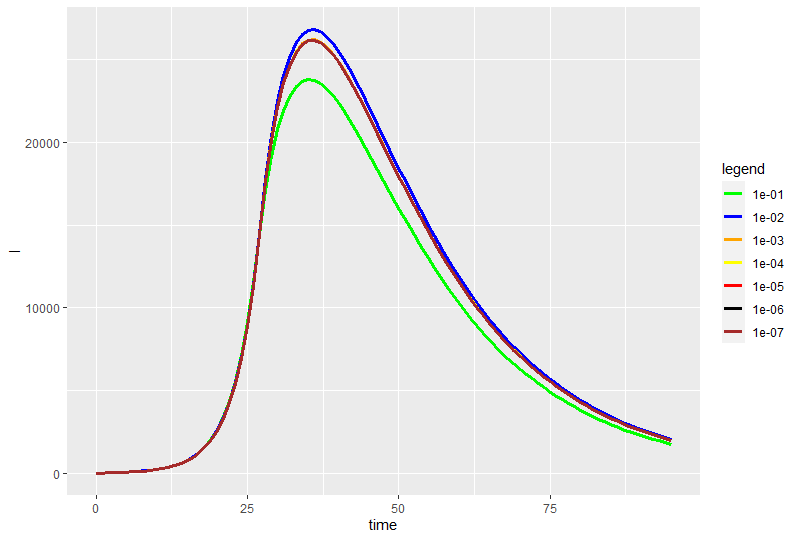
\includegraphics[width=0.7\linewidth]{./figures/tolerance_time_lsoda_no_event_R}
\caption{Time-discontinuity model tolerance study on the R version of LSODA without a cold start.}
\label{fig:tolerance_time_lsoda_no_event_R}
\end{figure}

\begin{figure}[H]
\centering
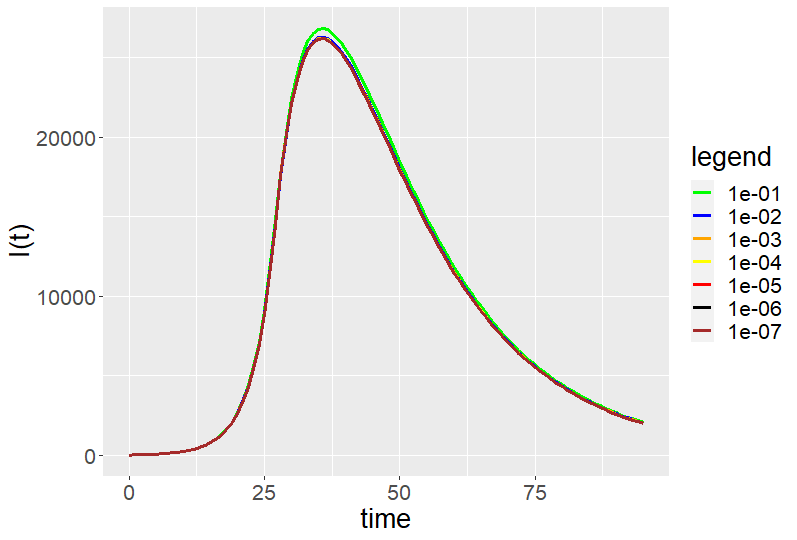
\includegraphics[width=0.7\linewidth]{./figures/tolerance_time_lsoda_with_event_R}
\caption{Time-discontinuity model tolerance study on the R version of LSODA with a cold start.}
\label{fig:tolerance_time_lsoda_with_event_R}
\end{figure}

From Figures $\ref{fig:tolerance_time_lsoda_no_event_R}$ and $\ref{fig:tolerance_time_lsoda_with_event_R}$, we can see that the introduction of discontinuity handling allows the solver to use coarser tolerances and still get a reasonable result; we need a tolerance at least as sharp as $10^{-3}$ without discontinuity handling but can use a tolerance as coarse as $10^{-2}$ with it. This supports the observation that the use of discontinuity handling when solving a discontinuous problem is advantageous. Also, using coarser tolerances leads to better efficiency, as we will see in Table $\ref{tab:tolerance_time_discontinuity_lsoda_R}$. 

\begin{table}[H]
\caption {The R LSODA time-dependent discontinuity model tolerance study - number of function evaluations} \label{tab:tolerance_time_discontinuity_lsoda_R} 
\begin{center}
\begin{tabular}{ c c c }
tolerance & no discontinuity handling & with discontinuity handling \\ 
1e-01 & 197 & 200 \\
1e-02 & 214 & 206 \\
1e-03 & 264 & 212 \\
1e-04 & 264 & 224 \\
1e-05 & 317 & 244 \\
1e-06 & 332 & 272 \\
1e-07 & 393 & 298 \\
\end{tabular}
\end{center}
\end{table}

From Table $\ref{tab:tolerance_time_discontinuity_lsoda_R}$, we see that for the coarser tolerances, the number of function evaluations is roughly the same. But with sharper tolerances, many more function evaluations are required and thus if we had a user-provided function that was expensive to evaluate, we would see clear reductions in computation times.

A similar number of function evaluations for the coarser tolerances should not distract us from the fact that the solver without discontinuity handling at these tolerances gives results that are not as accurate as the results obtained using the solver with discontinuity handling. The small differences of 3 function evaluations for the 0.1 tolerance case and 8 function evaluations in the 0.01 case do not excuse the fact that the solutions obtained when no discontinuity handling is employed are significantly less accurate.

\subparagraph{Time-dependent discontinuity LSODA tolerance study in Python}
In this section, we run the Python version of the LSODA solver with multiple tolerances with and without discontinuity handling. We note that the Python solvers give sufficiently accurate results in both cases apart from some small disagreements in the case where no discontinuity handling is employed but we will see how coarse we can choose the tolerance while still obtaining reasonably accurate results. We set both the relative and absolute tolerances to various values. We also look at efficiency data to see the decreases in the number of function evaluations.

\begin{figure}[H]
\centering
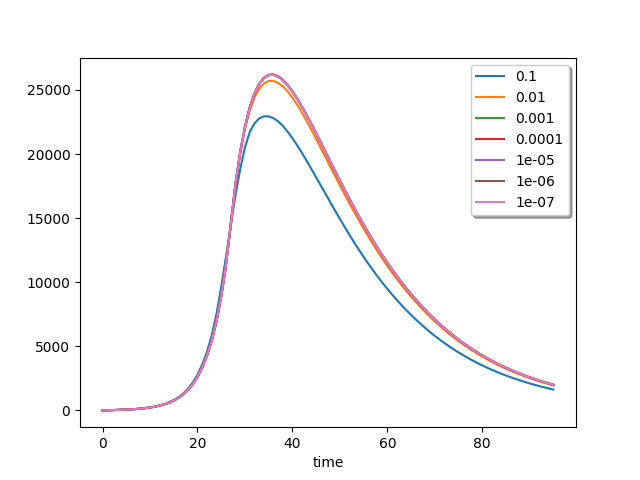
\includegraphics[width=0.7\linewidth]{./figures/tolerance_time_lsoda_no_event_py}
\caption{Time-dependent discontinuity model tolerance study on the Python version of LSODA without a cold start.}
\label{fig:tolerance_time_lsoda_no_event_py}
\end{figure}

\begin{figure}[H]
\centering
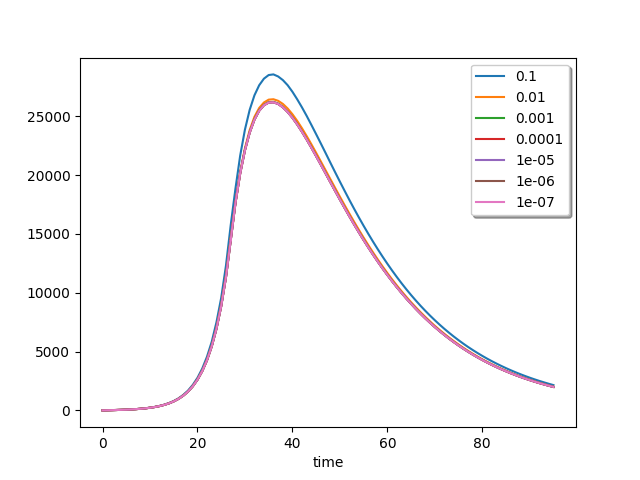
\includegraphics[width=0.7\linewidth]{./figures/tolerance_time_lsoda_with_event_py}
\caption{Time-dependent  discontinuity model tolerance study on the Python version of LSODA with a cold start.}
\label{fig:tolerance_time_lsoda_with_event_py}
\end{figure}

From Figures $\ref{fig:tolerance_time_lsoda_with_event_py}$ and $\ref{fig:tolerance_time_lsoda_no_event_py}$, we see that with the use of the discontinuity handling, a tolerance of $10^{-2}$ is enough to get a reasonably accurate result whereas a tolerance of $10^{-3}$ is needed otherwise. Also, the use of coarser tolerances leads to better efficiency, as can be seen in Table $\ref{tab:tolerance_time_discontinuity_lsoda_py}$.

\begin{table}[H]
\caption {Python LSODA time-dependent discontinuity model tolerance study - number of function evaluations} \label{tab:tolerance_time_discontinuity_lsoda_py} 
\begin{center}
\begin{tabular}{ c c c }
tolerance & no discontinuity handling & with discontinuity handling \\ 
0.1 & 79 & 86 \\
0.01 & 98 & 93 \\
0.001 & 156 & 116 \\
0.0001 & 185 & 146 \\
1e-05 & 259 & 186 \\
1e-06 & 283 & 228 \\
1e-07 & 361 & 272 \\
\end{tabular}
\end{center}
\end{table}
Again, in Table $\ref{tab:tolerance_time_discontinuity_lsoda_py}$, we see that that at coarse tolerances, the number of function evaluations is roughly the same. This similar number of function evaluations does not excuse the fact that the coarser tolerances are giving inaccurate solutions when discontinuity handling is not employed.

At sharper tolerances, where solutions of reasonable accuracy are obtained in all cases, the number of function evaluations is much smaller with discontinuity handling than without. There are 40 fewer function evaluations at 0.001 and 0.0001 and there are substantially fewer function evaluations for sharper tolerances. We note that if the function for the evaluation of the right-hand side of the ODE was more time-consuming, this reduced number of function evaluations will cause a significant decrease in the CPU times.

\subparagraph{Time-dependent  discontinuity LSODA tolerance study in Scilab}
In this section, we run the Scilab version of the LSODA solver with multiple tolerances with and without discontinuity handling. We will set both the relative and absolute tolerances to various values and see how coarse we can set the tolerance while still getting reasonably accurate results.

\begin{figure}[H]
\centering
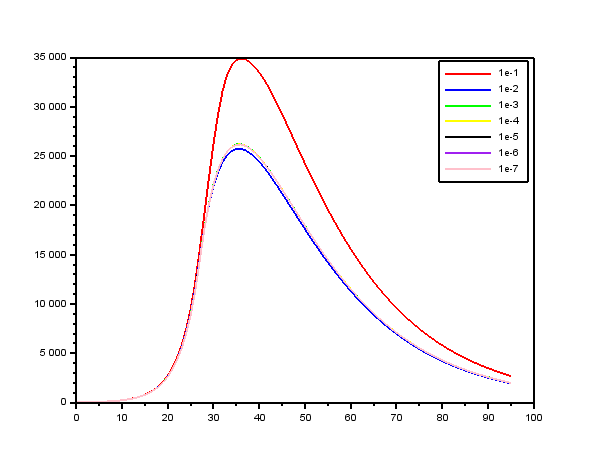
\includegraphics[width=0.7\linewidth]{./figures/tolerance_time_lsoda_no_event_sci}
\caption{Time-dependent  discontinuity model tolerance study on the Scilab version of lsoda without a cold start.}
\label{fig:tolerance_time_lsoda_no_event_sci}
\end{figure}

\begin{figure}[H]
\centering
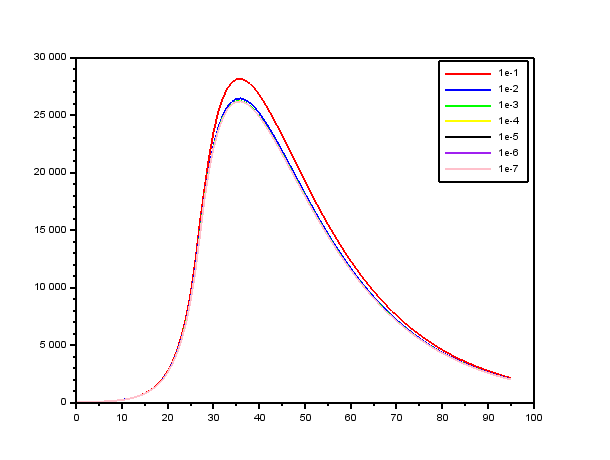
\includegraphics[width=0.7\linewidth]{./figures/tolerance_time_lsoda_with_event_sci}
\caption{Time-dependent  discontinuity model tolerance study on the Scilab version of lsoda with a cold start.}
\label{fig:tolerance_time_lsoda_with_event_sci}
\end{figure}

From Figures $\ref{fig:tolerance_time_lsoda_no_event_sci}$ and $\ref{fig:tolerance_time_lsoda_with_event_sci}$ we can see that for tolerances from $10^{-1}$ to $10^{-4}$, the Scilab version of LSODA without discontinuity handling does not yield reasonably accurate solutions but we are able to use a tolerance as coarse as $10^{-2}$ with discontinuity handling. 

It is interesting to see how inacurate the solution without discontinuity handling is at a tolerance of $10^{-1}$. We also note that this behavior is different from the R and the Python version LSODA but this may be due to the way Scilab handles the tolerances.

\begin{table}[H]
\caption {Scilab LSODA time-dependent discontinuity model tolerance study - number of function evaluations} 
\label{tab:tolerance_time_discontinuity_lsoda_scilab} 
\begin{center}
\begin{tabular}{ c c c }
tolerance & no discontinuity handling & with discontinuity handling \\ 
0.1 & 80 & 82 \\
0.01 & 98 & 92 \\
0.001 & 156 & 116 \\
1e-4 & 185 & 146 \\
1e-5 & 255 & 186 \\
1e-6 & 280 & 228 \\
1e-7 & 361 & 272 \\
\end{tabular}
\end{center}
\end{table}
Again, in Table $\ref{tab:tolerance_time_discontinuity_lsoda_scilab}$, we see that the number of function evaluations is roughly the same at coarser tolerances but that at sharp tolerances, where both types of computations give reasonably accurate solutions and thus allow for a fair comparison, the solver with discontinuity handling performs better than the solver without discontinuity handling. We can use up to 90 fewer function evaluations through the use of discontinuity handling. 

\subsubsection{Comparing solvers based on Runge-Kutta pairs across platforms for the time dependent discontinuity problem}
\subparagraph{Time dependent discontinuity model tolerance study on the R version of DOPRI5}
In this section, we use the R version of DOPRI5, which is the `ode45' method of the $ode$ function, with multiple tolerances with and without discontinuity handling. We will set both the relative and absolute tolerances to various values and see how coarse we can choose the tolerance while still getting reasonably accurate results. We also look at efficiency data to examine the number of function evaluations in each case.

\begin{figure}[H]
\centering
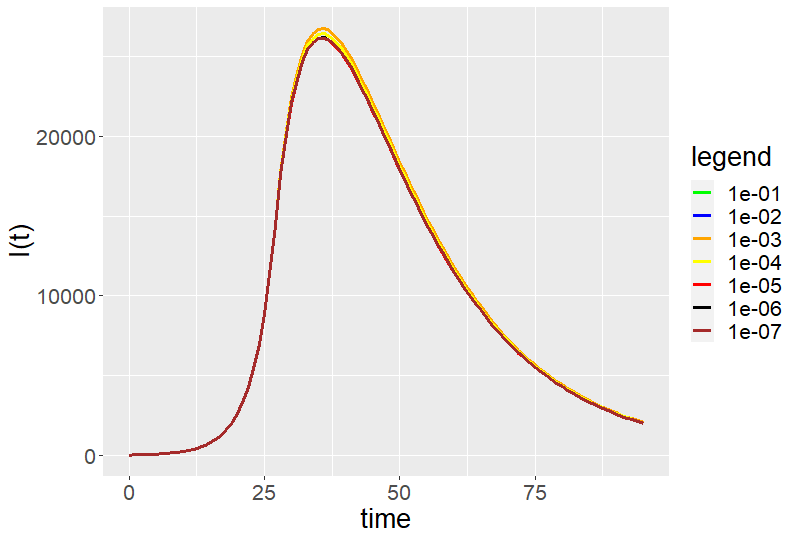
\includegraphics[width=0.7\linewidth]{./figures/tolerance_time_rk45_no_event_R}
\caption{Time-dependent discontinuity model tolerance study on the R version of DOPRI5 without discontinuity handling.}
\label{fig:tolerance_time_rk45_no_event_R}
\end{figure}

\begin{figure}[H]
\centering
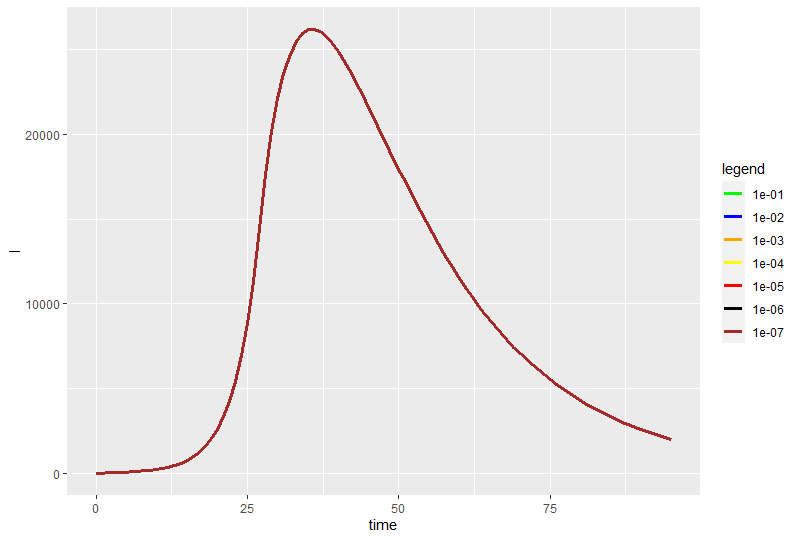
\includegraphics[width=0.7\linewidth]{./figures/tolerance_time_rk45_with_event_R}
\caption{Time-dependent discontinuity model tolerance study on the R version of DOPRI5 with discontinuity handling.}
\label{fig:tolerance_time_rk45_with_event_R}
\end{figure}

From Figures $\ref{fig:tolerance_time_rk45_no_event_R}$ and $\ref{fig:tolerance_time_rk45_with_event_R}$, we see that the addition of discontinuity handling lets us use a coarser tolerance and still get a reasonably accurate answer. Without discontinuity handling, we had to use $10^{-4}$ for both the absolute and relative tolerances but with discontinuity handling, we can use $10^{-1}$. 

However, as we will see in the Python version of DOPRI5, the results from Figures $\ref{fig:tolerance_time_rk45_no_event_R}$ and $\ref{fig:tolerance_time_rk45_with_event_R}$ are suspicious and stem from the fact that R is not using a proper interpolation scheme to produce the results. It is using an algorithm that depends on the selected output points and which affects efficiency and accuracy, as discussed in Section $\ref{subsection:solution_output_points_impl}$. 

\begin{table}[H]
\caption {The R DOPRI5 time-dependent discontinuity model tolerance study - number of function evaluations} \label{tab:tolerance_time_discontinuity_rk45_R} 
\begin{center}
\begin{tabular}{ c c c }
tolerance & no discontinuity handling & with discontinuity handling\\ 
1e-01 & 572 & 574 \\
1e-02 & 572 & 574 \\
1e-03 & 572 & 574 \\
1e-04 & 612 & 574 \\
1e-05 & 692 & 587 \\
1e-06 & 735 & 599 \\
1e-07 & 926 & 702 \\
\end{tabular}
\end{center}
\end{table}

Table $\ref{tab:tolerance_time_discontinuity_rk45_R}$ also confirms our suspicions since, at coarser tolerances, $10^{-1}$ to $10^{-3}$, the number of function evaluations does not change at all. This indicates that something else, not the tolerance nor the discontinuity, is the limiting factor for the number of function evaluations and that this other factor leads to a need for around 572 or 574 function evaluations.

We suspect that the R DOPRI5 version is not using an appropriate interpolation scheme to evaluate the numerical solution and that it is integrating using the output points to determine the step-size. We therefore perform the following experiment where we specify a smaller set of output points with the points further spaced out from each other.

\begin{figure}[H]
\centering
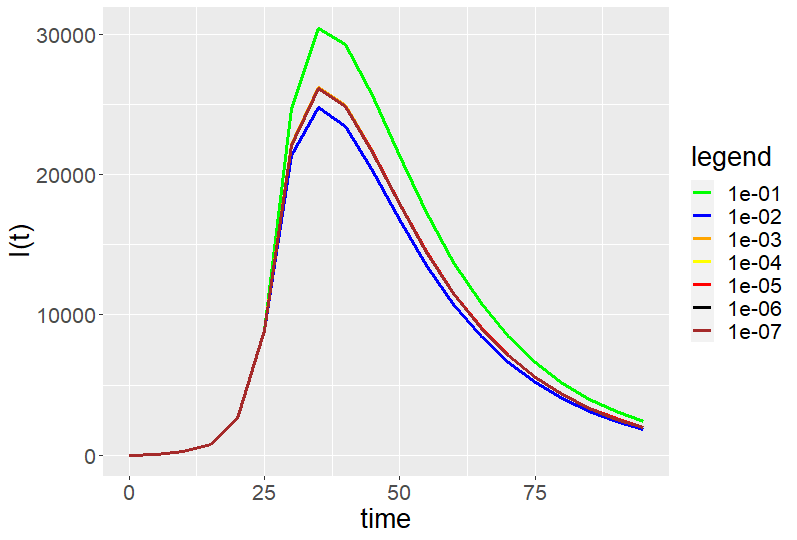
\includegraphics[width=0.7\linewidth]{./figures/tolerance_time_rk45_further_no_event_R}
\caption{Time-dependent discontinuity model tolerance study on the R version of DOPRI5 without discontinuity handling and with output points more spaced out.}
\label{fig:tolerance_time_rk45_further_no_event_R}
\end{figure}

\begin{figure}[H]
\centering
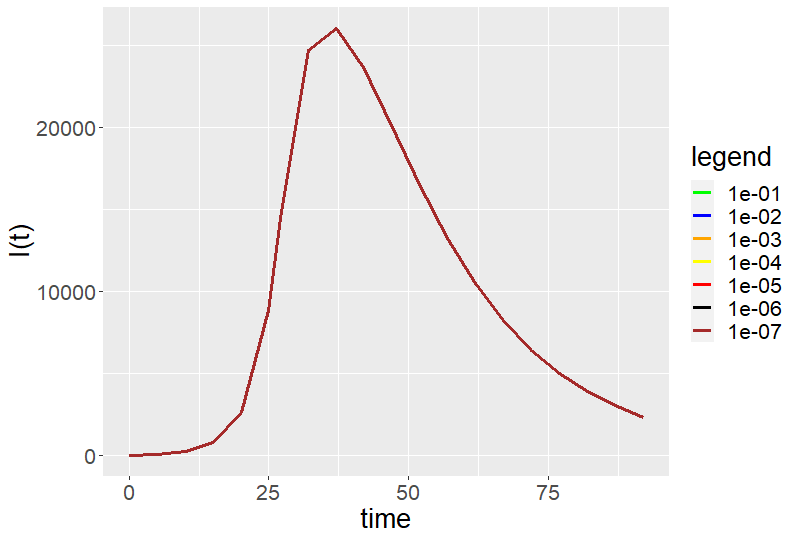
\includegraphics[width=0.7\linewidth]{./figures/tolerance_time_rk45_further_with_event_R}
\caption{Time-dependent discontinuity model tolerance study on the R version of DOPRI5 with discontinuity handling and with output points more spaced out.}
\label{fig:tolerance_time_rk45_further_with_event_R}
\end{figure}

From Figures $\ref{fig:tolerance_time_rk45_further_no_event_R}$ and $\ref{fig:tolerance_time_rk45_further_with_event_R}$, we can now see a more significant change in the solution when the output points are further spaced out. Also, we see in Table $\ref{tab:tolerance_time_discontinuity_rk45_further_R}$ that the number of function evaluations actually changes with the tolerance.

Using these two figures, we also see that discontinuity handling is allowing us to use coarser tolerances. We can even use  a tolerance of $10^{-1}$ with discontinuity handling while getting a reasonably accurate result, whereas, without discontinuity handling, we need to use a tolerance of $10^{-3}$ or sharper to get a reasonably accurate answer.

\begin{table}[H]
\caption {R DOPRI5 time-dependent discontinuity model tolerance study with spaced out output points - number of function evaluations} \label{tab:tolerance_time_discontinuity_rk45_further_R} 
\begin{center}
\begin{tabular}{ c c c }
tolerance & no discontinuity handling & with discontinuity handling \\ 
1e-01 & 116 & 112 \\
1e-02 & 142 & 125 \\
1e-03 & 168 & 131 \\
1e-04 & 246 & 162 \\
1e-05 & 352 & 235 \\
1e-06 & 614 & 349 \\
1e-07 & 796 & 542 \\
\end{tabular}
\end{center}
\end{table}

Our analysis of Table $\ref{tab:tolerance_time_discontinuity_rk45_further_R}$ begins by noting that the set of output points is no longer a limiting factor. We can see that the number of function evaluations changes with the tolerance and this indicates that the tolerance is controlling the step-size. This confirms our suspicion that the R implementation of DOPRI5 is not using an appropriate scheme for treating the output points. Instead, it is allowing the output points determine the step-size and thus dictate the efficiency of the solver.

Regarding the accuracy of the solver as we coarsen the tolerance we can see from Figures $\ref{fig:tolerance_time_rk45_further_no_event_R}$ and $\ref{fig:tolerance_time_rk45_further_with_event_R}$ that even at a tolerance of $10^{-1}$, the solver with the discontinuity handling is still able to produce reasonably accurate solutions whereas it requires a tolerance of $10^{-3}$ for the solver without discontinuity handling.

The new table, Table $\ref{tab:tolerance_time_discontinuity_rk45_further_R}$, does offer some more insights. Again we can see that at coarser tolerances, the decrease in the number of function evaluations when discontinuity handling is employed is small but as the tolerance is sharpened, the number of function evaluations when discontinuity handling is employed decreases significantly. The relatively similar number of function evaluations at the coarser tolerances must be viewed in light of the fact that the solver without discontinuity handling is not getting a reasonably accurate answer. 

\subparagraph{Time dependent discontinuity model tolerance study on the Python version of DOPRI5}
In this section, we run the Python version of DOPRI5, which is aliased under 'RK45' from the $solver\_ivp$ function, with multiple tolerances, with and without discontinuity handling. We will set both the relative and absolute tolerances to various values and see how coarse we can choose the tolerance while still obtaining reasonably accurate results. We also look at efficiency data to determine  the number of function evaluations in each case.

\begin{figure}[H]
\centering
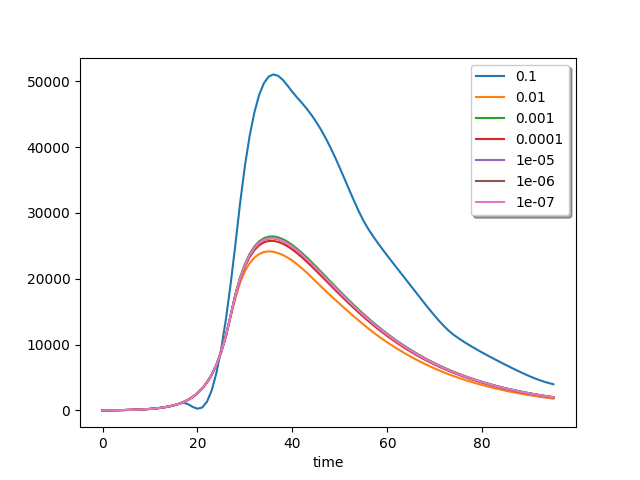
\includegraphics[width=0.7\linewidth]{./figures/tolerance_time_rk45_no_event_py}
\caption{Time-dependent discontinuity model tolerance study on the Python version of DOPRI5 without discontinuity handling.}
\label{fig:tolerance_time_rk45_no_event_py}
\end{figure}

\begin{figure}[H]
\centering
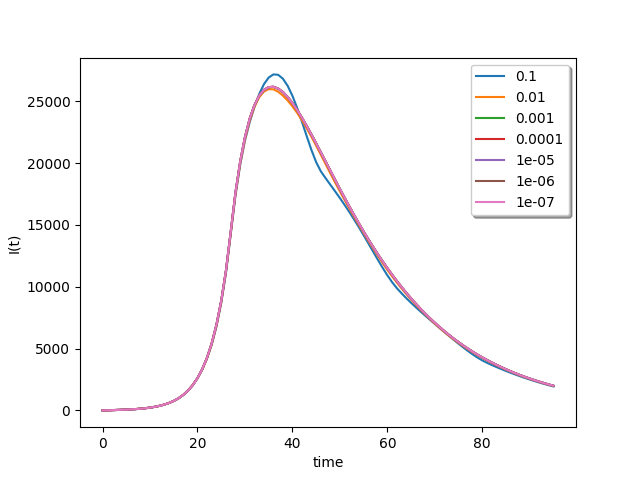
\includegraphics[width=0.7\linewidth]{./figures/tolerance_time_rk45_with_event_py}
\caption{Time-dependent discontinuity model tolerance study on the Python version of DOPRI5 with discontinuity handling.}
\label{fig:tolerance_time_rk45_with_event_py}
\end{figure}

From Figures $\ref{fig:tolerance_time_rk45_with_event_py}$ and $\ref{fig:tolerance_time_rk45_no_event_py}$, we can see clear differences in the computed solutions at different tolerance values. From studying Python's $solve\_ivp$ interface and source code, we note that Python is using interpolation
to treat the output points.

We then compare the Python version of DOPRI5 with and without discontinuity handling. We can see that the use of discontinuity handling allows us to use coarser tolerances while obtaining reasonably accurate results. We see that we need a tolerance of $10^{-5}$ or sharper to get reasonably accurate solutions without discontinuity handling while a tolerance of $10^{-2}$ is small enough when discontinuity handling is employed. We will also see in Table $\ref{tab:tolerance_time_discontinuity_rk45_py}$ that the solver with discontinuity handling is much more efficient.


\begin{table}[H]
\caption {Python DOPRI5 time-dependent discontinuity model tolerance study - number of function evaluations} \label{tab:tolerance_time_discontinuity_rk45_py} 
\begin{center}
\begin{tabular}{ c c c }
tolerance & no discontinuity handling & with discontinuity handling \\ 
0.1 & 68 & 70 \\
0.01 & 86 & 88 \\
0.001 & 146 & 124 \\
0.0001& 224 & 172 \\
1e-05 & 326 & 250 \\
1e-06 & 488 & 370 \\
1e-07 & 752 & 568 \\
\end{tabular}
\end{center}
\end{table}

From Table $\ref{tab:tolerance_time_discontinuity_rk45_py}$, we see that at coarser tolerances, the number of function evaluations is greater with the discontinuity handling than without discontinuity handling but we must point out that DOPRI5 at coarse tolerances gives very inaccurate results; the errors are too large to excuse the small gain in efficiency.

At sharper tolerances where we get reasonably accurate results both with and without discontinuity handling, and thus a fair comparison can be done, we can see that the solver that uses discontinuity handling performs much better. At a tolerance of $10^{-5}$ or sharper, the decrease in the number of function evaluations is 75 or more.

\subparagraph{Time dependent discontinuity model tolerance study on the Scilab version of RKF45}
In this section, we run the Scilab version of RKF45 aliased as `rkf' in the $ode$ function with different tolerances. We note that the default tolerance for the Scilab `rkf' function was not sufficiently small to solve the problem to reasonable accuracy without discontinuity handling but using cold starts did solve the problem even with that default tolerance. 

By running `rkf' at various tolerances, we will show that it can also compute reasonably accurate solutions at sharper tolerances without discontinuity handling. Thus the anomaly we saw in Section $\ref{subsection:naive_time_problem}$ occurred entirely because the solver has a coarser default tolerance than the other methods.

We will also see that using discontinuity handling leads to the use of fewer function evaluations which, given a more complex problem, would result in a significant improvement in computation times.

\begin{figure}[H]
\centering
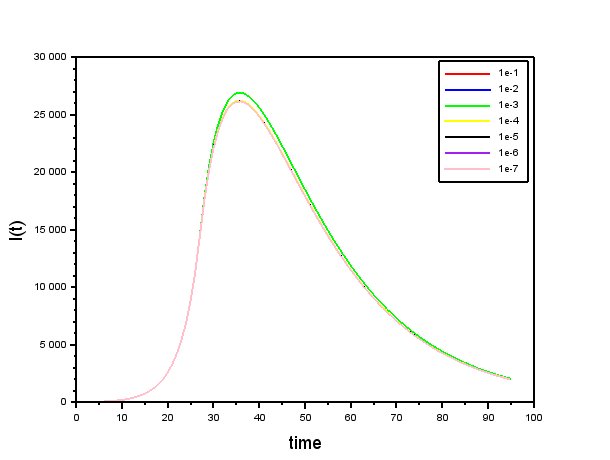
\includegraphics[width=0.7\linewidth]{./figures/tolerance_time_rk45_no_event_sci}
\caption{Time discontinuity model tolerance study on the Scilab version of RKF45 without discontinuity handling.}
\label{fig:tolerance_time_rk45_no_event_sci}
\end{figure}

\begin{figure}[H]
\centering
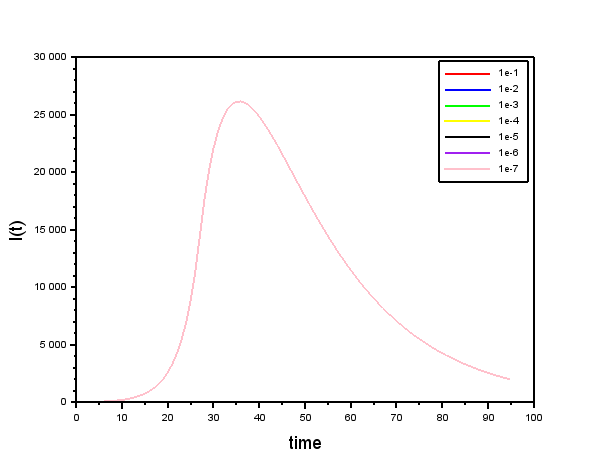
\includegraphics[width=0.7\linewidth]{./figures/tolerance_time_rk45_with_event_sci}
\caption{Time discontinuity model tolerance study on the Scilab version of RKF45 with discontinuity handling.}
\label{fig:tolerance_time_rk45_with_event_sci}
\end{figure}

We see from Figure $\ref{fig:tolerance_time_rk45_no_event_sci}$ that using $10^{-4}$ for both the absolute and the relative tolerance gives reasonably accurate answers and that anything coarser leads to somewhat inaccurate solutions. We then recall that the relative tolerance defaults to $10^{-3}$ and the absolute tolerance defaults to $10^{-4}$ for `rkf' which is slightly coarser than what is needed to get a reasonably accurate solution.

Figure $\ref{fig:tolerance_time_rk45_with_event_sci}$ is also interesting as it seems to indicate that a tolerance of $10^{-1}$ is enough to get a reasonably accurate solution with discontinuity handling. This is surprising but consistent with our observations for the R and Python Runge-Kutta pairs.

\begin{table}[H]
\caption {Scilab RKF45 time-dependent discontinuity model tolerance study - number of function evaluations} 
\label{tab:tolerance_time_discontinuity_rk45_scilab} 
\begin{center}
\begin{tabular}{ c c c }
tolerance & no discontinuity handling & with discontinuity handling\\ 
0.1 & 577 & 584 \\
0.01 & 577 & 584 \\
0.001 & 583 & 584 \\
1e-4 & 641 & 590 \\
1e-5 & 674 & 608 \\
1e-6 & 847 & 764 \\
1e-7 & 924 & 830 \\
\end{tabular}
\end{center}
\end{table}
We can see from Table $\ref{tab:tolerance_time_discontinuity_rk45_scilab}$ that the Scilab RKF45 method is not using interpolation to treat the output points. We can make this conclusion because at extremely coarse tolerances, it is using the same number of function evaluations despite the tolerance. There is also no difference with and without discontinuity handling. We also note that a change in the tolerance did not lead to a change in the number of function evaluations and thus something else is determining the number of function evaluations. Doing the same experiment with the points further spaced out shows us that it is the spacing of the output points that is causing the issue. We thus replicate the experiments in the previous sections with the output points more spread out.
\begin{figure}[H]
\centering
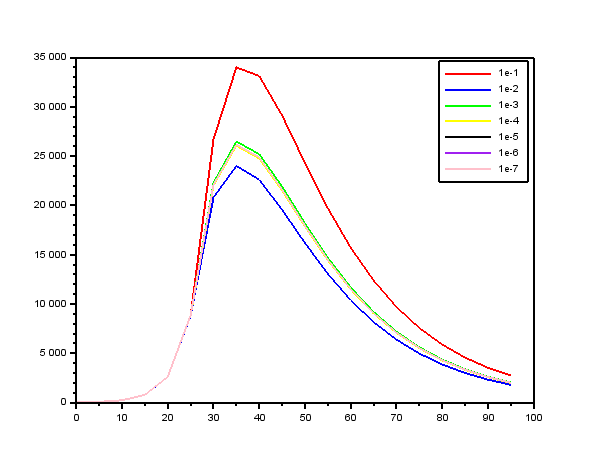
\includegraphics[width=0.7\linewidth]{./figures/tolerance_time_rkf_further_no_event_sci}
\caption{Time discontinuity model tolerance study on the Scilab version of RKF45 without discontinuity handling.}
\label{fig:tolerance_time_rkf_further_no_event_sci}
\end{figure}

\begin{figure}[H]
\centering
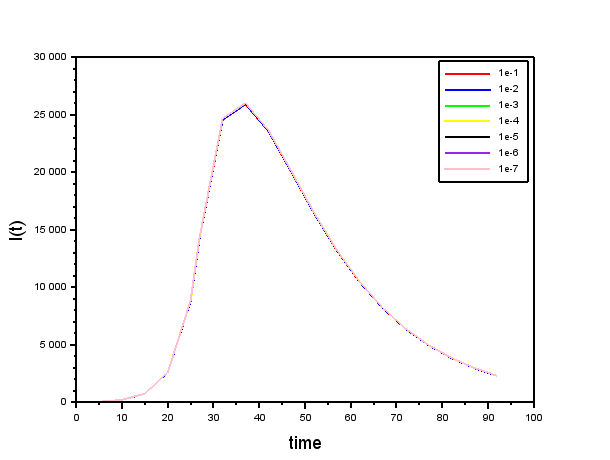
\includegraphics[width=0.7\linewidth]{./figures/tolerance_time_rkf_further_with_event_sci}
\caption{Time discontinuity model tolerance study on the Scilab version of RKF45 with discontinuity handling.}
\label{fig:tolerance_time_rkf_further_with_event_sci}
\end{figure}

Figures $\ref{fig:tolerance_time_rkf_further_no_event_sci}$ and $\ref{fig:tolerance_time_rkf_further_with_event_sci}$ show a clear indication regarding why discontinuity handling is important. We can see that without it, we need a tolerance of $10^{-3}$ to get reasonably accurate results but with the discontinuity handling, we can use a tolerance of $10^{-1}$. The impact on the number of function evaluations, shown in Table $\ref{tab:tolerance_time_discontinuity_rk45_spaced_out_scilab}$, is clear.

\begin{table}[H]
\caption {Scilab RKF45 with spaced out ouptut points, time-dependent discontinuity model, tolerance study - number of function evaluations} 
\label{tab:tolerance_time_discontinuity_rk45_spaced_out_scilab} 
\begin{center}
\begin{tabular}{ c c c }
tolerance & no discontinuity handling & with discontinuity handling\\ 
0.1 & 133 & 134 \\
0.01 & 166 & 152 \\
0.001 & 208 & 176 \\
1e-4 & 322 & 254 \\
1e-5 & 417 & 338 \\
1e-6 & 606 & 482 \\
1e-7 & 864 & 704 \\
\end{tabular}
\end{center}
\end{table}

Table $\ref{tab:tolerance_time_discontinuity_rk45_spaced_out_scilab}$ shows that the number of function evaluations, when discontinuity handling is employed, is smaller. We also note that at coarse tolerances, the number of function evaluations is similar but that at those tolerances, the solver without discontinuity handling is not obtaining reasonably accurate results. We can thus conclude that using discontinuity handling lets us use coarser tolerances and leads to a smaller number of function evaluations while improving accuracy.


\subparagraph{Time-dependent discontinuity model tolerance study on the Matlab version of DOPRI5}
We perform the same experiment using $ode45$ in Matlab. We set both the absolute and relative tolerance to various values and examine how the solver perform. We recall that, using the default tolerance, $ode45$ did not give a reasonably accurate solution. We also recall that $ode45$ did not have a smaller default tolerance than $ode15s$. In this section, we show that with a sharper tolerance, $ode45$ is also capable of solving the problem without discontinuity handling but we will see that it is more efficient with discontinuity handling. Discontinuity handling will, again, allow us to use coarser tolerances and still obtain reasonably accurate solutions.

\begin{figure}[H]
\centering
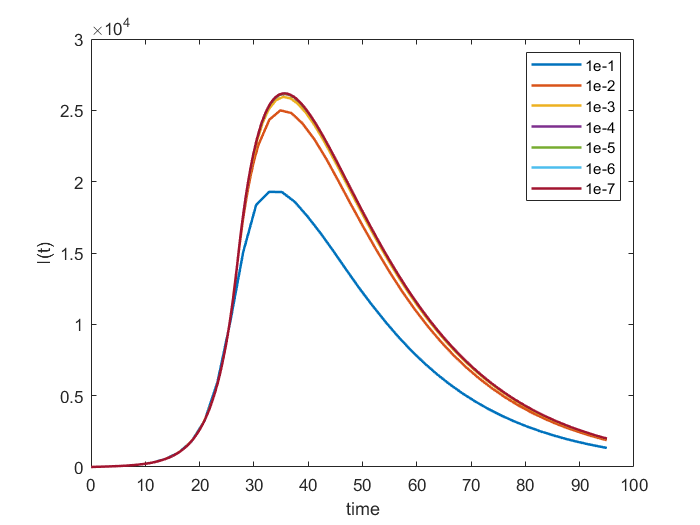
\includegraphics[width=0.7\linewidth]{./figures/tolerance_time_rk45_no_event_matlab}
\caption{Time discontinuity model tolerance study on the Matlab version of DOPRI5 without discontinuity handling.}
\label{fig:tolerance_time_rk45_no_event_matlab}
\end{figure}

We first note from Figure $\ref{fig:tolerance_time_rk45_no_event_matlab}$ that at sufficiently sharp tolerances, we can get a reasonably accurate answer without discontinuity handling whereas the default tolerances did not give a reasonably accurate solution.

\begin{figure}[H]
\centering
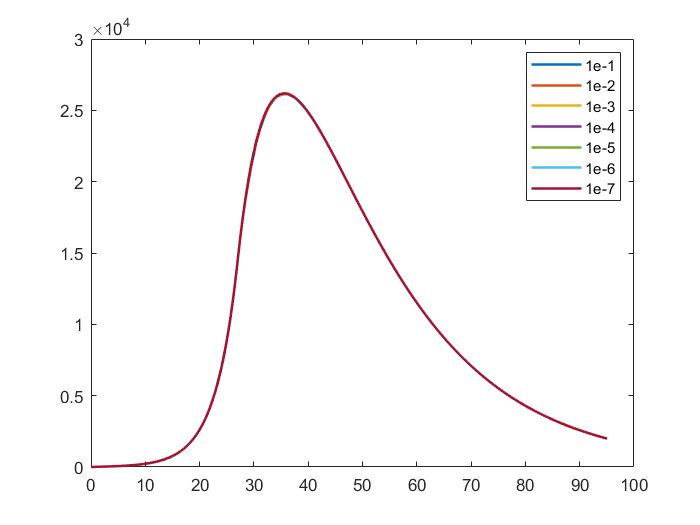
\includegraphics[width=0.7\linewidth]{./figures/tolerance_time_rk45_with_event_matlab}
\caption{Time discontinuity model tolerance study on the Matlab version of DOPRI5 with discontinuity handling.}
\label{fig:tolerance_time_rk45_with_event_matlab}
\end{figure}

From Figures $\ref{fig:tolerance_time_rk45_no_event_matlab}$ and $\ref{fig:tolerance_time_rk45_with_event_matlab}$ we see that discontinuity handling allows us to use coarser tolerances while still getting a reasonably accurate solution. We note that we could use a tolerance of $10^{-1}$ with discontinuity handling but we had to use a tolerance of $10^{-3}$ to get a reasonably accurate solution when no discontinuity handling is employed. We will also see that discontinuity handling allows the solver to use fewer function evaluations in Table $\ref{tab:tolerance_time_discontinuity_rk45_matlab}$.

\begin{table}[H]
\caption {The Matlab DOPRI5 time-dependent discontinuity model tolerance study - number of function evaluations} 
\label{tab:tolerance_time_discontinuity_rk45_matlab} 
\begin{center}
\begin{tabular}{ c c c }
tolerance & no discontinuity handling & with discontinuity handling\\ 
0.1 & 85 & 146 \\
0.01 & 121 & 146 \\
0.001 & 169 & 158 \\
0.0001 & 229 & 200 \\
1e-05 & 355 & 302 \\
1e-06 & 547 & 446 \\
1e-07 & 823 & 692 \\
\end{tabular}
\end{center}
\end{table}

Table $\ref{tab:tolerance_time_discontinuity_rk45_matlab}$ show that at coarser tolerances the solver without discontinuity handling uses fewer function evaluations. However, at these tolerances, the solver does not give a reasonably accurate solution. At shaper tolerances, where the solver without discontinuity handling gives a reasonably accurate solution, the number of function evaluations for the solver with discontinuity handling is lower.
